% ***********************************************************
% ******************* MATH HEADER ************************
% ***********************************************************
% Version Template 1.0
\documentclass[12pt]{article}
\usepackage{amsmath, amsthm, amssymb, float, graphicx, tensor, commath, mdframed, xcolor, tikz, pgfplots}
\pgfplotsset{compat=1.18}
\usepackage[bottom]{footmisc}
\usepackage[justification=centering]{caption}
\usepackage[letterpaper,margin=1in,bottom=0.7in]{geometry}
\usepackage{enumerate, cancel}

% Redefining vector and unit vector commands
\newcommand{\vect}[1]{\ensuremath{\mathbf{#1}}} % for vectors
\newcommand{\unitvect}[1]{\ensuremath{\mathbf{\hat{#1}}}} % for unit vectors

% Custom preamble for sheet title and course information
\newcommand{\SheetTitle}[3]{
  {\noindent\Huge\bf  \\[0.5\baselineskip] {\fontfamily{cmr}\selectfont  Problem Set I}}\\[2\baselineskip] % Enter Title Here
  { {\bf \fontfamily{cmr}\selectfont #1}\\ {\textit{\fontfamily{cmr}\selectfont \today}}}    ~~~~~~~~~~~~~~~~~~~~~~~~~~~~~~~~~~~~~~~~~~~~~~~~~~~~~~~~~~~~~~~~~~~~     {\large \textsc{Enter Name}\thanks{With #3}} \\
  {Enter Professor Name}
  \\[1.4\baselineskip]}

\renewcommand*{\qedsymbol}{$\blacksquare$}

% Environment for solutions using the proof environment
\newenvironment{s}
  {\begin{mdframed}\begin{proof}[Solution.]}
  {\end{proof}\end{mdframed}}

% Set the theorem style to "definition" (upright text)
\theoremstyle{definition}

% Define the problem environment with upright text
\newtheorem{p}{Problem}

% Define solution environment with a box
\newenvironment{solution}
  {\begin{mdframed}[linewidth=0.5pt, roundcorner=10pt, linecolor=black]\begin{proof}[\bfseries Solution]}
  {\qedhere\end{proof}\end{mdframed}}
  
\definecolor{bluee}{HTML}{046DE9}
\definecolor{redd}{HTML}{CE1F15}
\definecolor{greenn}{HTML}{28AC3C}

\renewcommand{\footnoterule}{%
    \kern -3pt
    \hrule width 0.635\textwidth height 0.5pt
    \kern 2pt
}



% Define the remark environment with bold heading and italicized body


% Define the boxed remark environment with bold title and italicized content
\newenvironment{remark}
  {\begin{mdframed}[linewidth=0.5pt, roundcorner=10pt, linecolor=black]
   \textbf{Remark.} \itshape}
  {\end{mdframed}}

% ***********************************************************
% ********************** END HEADER *************************
% ***********************************************************

\begin{document}

% Change the title, course, author, and professor details
\SheetTitle{Problem Set Title}{Course Name}{Author Name}

\section{Section Title}

% Example of a problem
\vspace{0.9cm}
\begin{p}
  Problem statement here.
\end{p}

\begin{solution}
  Solution goes here. Use the \emph{italic} or \textbf{bold} text as needed.
  
  You can add figures (Fig.~\ref{fig:example}) with captions and labels:
  \begin{figure}[H]
    \centering
    \includegraphics[width=0.5\textwidth]{figures/example.jpg}
    \caption{\emph{Caption for the example figure.}}
    \label{fig:example}
  \end{figure}

  Continue with the rest of the solution. For equations, you can use:
  \begin{equation}
    E = mc^2
  \end{equation}

  or 

  \begin{align*}
    E &= mc^2 \\
    F &= ma
  \end{align*} \\

  You can create graphs with the \texttt{tikz} package, or use the \texttt{pgfplots} package for plots.\\

  \begin{figure}[H]
    \centering
    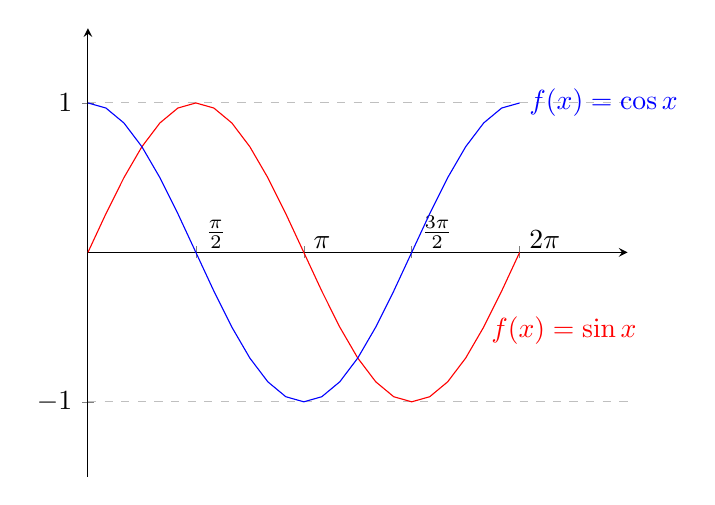
\begin{tikzpicture}
        \begin{axis}[
            clip=false,
            xmin=0, xmax=2.5*pi,
            ymin=-1.5, ymax=1.5,
            axis lines=middle,
            xtick={0, pi/2, pi, 3*pi/2, 2*pi},
            xticklabels={$0$, $\frac{\pi}{2}$, $\pi$, $\frac{3\pi}{2}$, $2\pi$},
            xticklabel style={anchor=south west},
            ymajorgrids=true,
            grid style=dashed
        ]
            \addplot[domain=0:2*pi, red]{sin(deg(x))}
            node[right, pos=0.9]{$f(x)=\sin x$};
            \addplot[domain=0:2*pi, blue]{cos(deg(x))}
            node[right, pos=1]{$f(x)=\cos x$};
        \end{axis}
    \end{tikzpicture}
    \caption{Sine and Cosine functions}
    \label{fig:sine_cosine_plot}
  \end{figure}


  
  Add more text here, or conclude your solution.

\end{solution}

\begin{remark}
  Remarks can be added at the beginning, end, or in the solution.
\end{remark}

\vspace{\lineskip}

\begin{proof}
  Proofs can be added at the beginning, end, or in the solution.
\end{proof}

% You can copy the above block for multiple problems and solutions.

\footnotetext{Collaborators or other acknowledgments can be added here.}
\end{document}